\title{Colors of image noise}


\section{White Gaussian noise}

Everybody knows about white Gaussian noise


\includegraphics{white.png}
%SCRIPT plambda zero:512x512 randg | qauto -p 0.1 - white.png &


White Gaussian noise is famous because it has very nice properties:

\begin{enumerate}
	\item It is easy to generate using pseudorandom numbers
	\item Each pixel is an independent, identically distributed Normal
		variable
	\item The discrete Fourier, Hartley and Cosine transforms are also
		white Gaussian noise (except for the obvious symmetries)
	\item In particular, the power spectrum is mostly flat
	\item Applying a linear filter renders the pixel values
		non-independent, but they are still Normal and identically
		distributed.
\end{enumerate}


Some properties of dubious convenience:
\begin{enumerate}
	\item The mean is zero, thus it cannot be directly represented as
		a positive-valued image
	\item Worse, the pixel values are not bounded, thus it has a-priori
		infinite dynamic range.
	\item When you see it from far away (zooming-out), it disappears.
\end{enumerate}



Statistics of white gaussian noise and its DFT:

\begin{tabular}{cccc}
	
\includegraphics{w256.png} &
	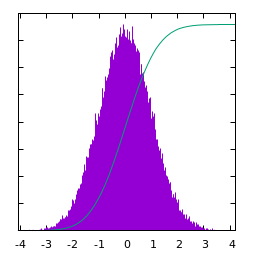
\includegraphics{w256_h.png} &
	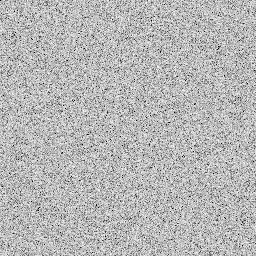
\includegraphics{w256_f.png} &
	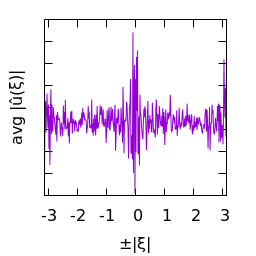
\includegraphics{w256_p.png} \\
	$u(x)$ &
	histogram of~$u$ &
	$\log|\hat u(\xi)|$ &
	average spectral profile
\end{tabular}
%SCRIPT plambda zero:256x256 randg -o w256.tiff
%SCRIPT qauto -p 0.1 w256.tiff w256.png &
%SCRIPT plambda w256.tiff 'x%a x%i - 300 / >1 x <1 / round <1 *' | ghisto -p | \
%SCRIPT        sed 's/cairo/cairo enhanced font "Verdana,8" size 256,256/' |\
%SCRIPT        gnuplot > w256_h.png &
%SCRIPT fft<w256.tiff|fftshift|plambda 'vnorm 1 + log'|qauto -p .1 - w256_f.png&
%SCRIPT (printf 'set term pngcairo size 256,256\nset format y ""\nset xlabel "±|ξ|"\nset ylabel "avg |û(ξ)|"\n'; fft <w256.tiff|fftshift|plambda 'vnorm'|cline nan|sed 's/data//g')|gnuplot > w256_p.png &


\section{Blurred white Gaussian noise}

White gaussian noise blurred by a small gaussian kernel:

\begin{tabular}{cccc}
	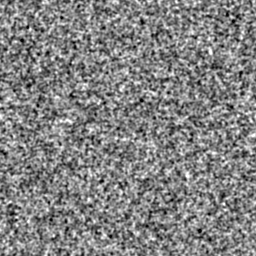
\includegraphics{b256.png} &
	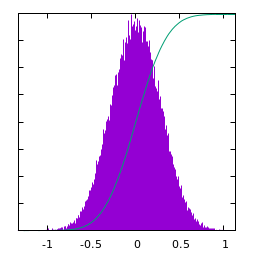
\includegraphics{b256_h.png} &
	
\includegraphics{b256_f.png} &
	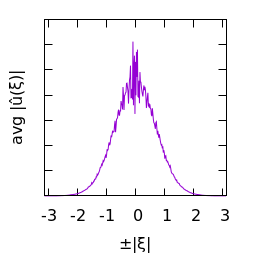
\includegraphics{b256_p.png} \\
	$u(x)$ &
	histogram of~$u$ &
	$\log|\hat u(\xi)|$ &
	average spectral profile
\end{tabular}
%SCRIPT plambda zero:256x256 randg |blur g 1 - b256.tiff
%SCRIPT qauto -p 0.1 b256.tiff b256.png &
%SCRIPT plambda b256.tiff 'x%a x%i - 300 / >1 x <1 / round <1 *' | ghisto -p | \
%SCRIPT        sed 's/cairo/cairo enhanced font "Verdana,8" size 256,256/' | \
%SCRIPT        gnuplot > b256_h.png &
%SCRIPT fft<b256.tiff|fftshift|plambda 'vnorm 1 + log'|qauto -p .1 - b256_f.png&
%SCRIPT (printf 'set term pngcairo size 256,256\nset format y ""\nset xlabel "±|ξ|"\nset ylabel "avg |û(ξ)|"\n'; fft <b256.tiff|fftshift|plambda 'vnorm'|cline nan|sed 's/data//g')|gnuplot > b256_p.png &



White gaussian noise blurred by a larger gaussian kernel:

\begin{tabular}{cccc}
	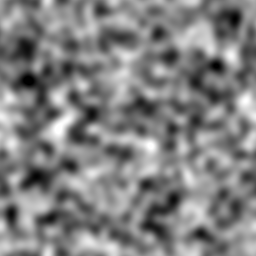
\includegraphics{B256.png} &
	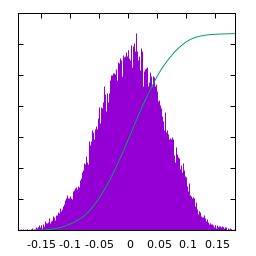
\includegraphics{B256_h.png} &
	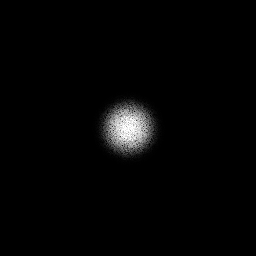
\includegraphics{B256_f.png} &
	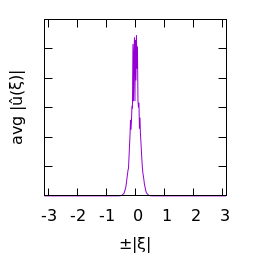
\includegraphics{B256_p.png} \\
	$u(x)$ &
	histogram of~$u$ &
	$\log|\hat u(\xi)|$ &
	average spectral profile
\end{tabular}
%SCRIPT plambda zero:256x256 randg |blur g 5 - B256.tiff
%SCRIPT qauto -p 0.1 B256.tiff B256.png &
%SCRIPT plambda B256.tiff 'x%a x%i - 300 / >1 x <1 / round <1 *' | ghisto -p | \
%SCRIPT        sed 's/cairo/cairo enhanced font "Verdana,8" size 256,256/' | \
%SCRIPT        gnuplot > B256_h.png &
%SCRIPT fft<B256.tiff|fftshift|plambda 'vnorm 1 + log'|qauto -p .1 - B256_f.png&
%SCRIPT (printf 'set term pngcairo size 256,256\nset format y ""\nset xlabel "±|ξ|"\nset ylabel "avg |û(ξ)|"\n'; fft <B256.tiff|fftshift|plambda 'vnorm'|cline nan|sed 's/data//g')|gnuplot > B256_p.png &



White gaussian noise blurred by a Cauchy kernel:

\begin{tabular}{cccc}
	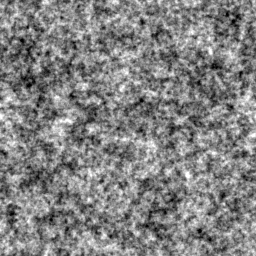
\includegraphics{c256.png} &
	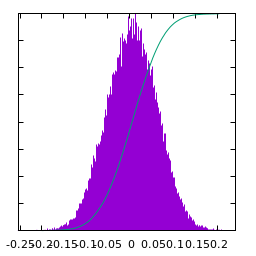
\includegraphics{c256_h.png} &
	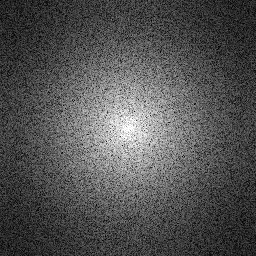
\includegraphics{c256_f.png} &
	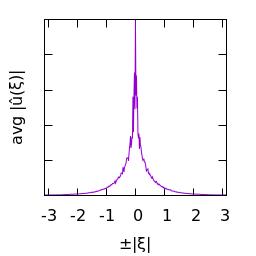
\includegraphics{c256_p.png} \\
	$u(x)$ &
	histogram of~$u$ &
	$\log|\hat u(\xi)|$ &
	average spectral profile
\end{tabular}
%SCRIPT plambda zero:256x256 randg |blur c 1 - c256.tiff
%SCRIPT qauto -p 0.1 c256.tiff c256.png &
%SCRIPT plambda c256.tiff 'x%a x%i - 300 / >1 x <1 / round <1 *' | ghisto -p | \
%SCRIPT        sed 's/cairo/cairo enhanced font "Verdana,8" size 256,256/' |\
%SCRIPT        gnuplot > c256_h.png &
%SCRIPT fft<c256.tiff|fftshift|plambda 'vnorm 1 + log'|qauto -p .1 - c256_f.png&
%SCRIPT (printf 'set term pngcairo size 256,256\nset format y ""\nset xlabel "±|ξ|"\nset ylabel "avg |û(ξ)|"\n'; fft <c256.tiff|fftshift|plambda 'vnorm'|cline nan|sed 's/data//g')|gnuplot > c256_p.png &



White gaussian noise blurred by a Laplace kernel:

\begin{tabular}{cccc}
	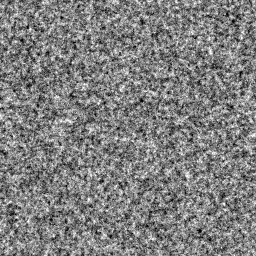
\includegraphics{l256.png} &
	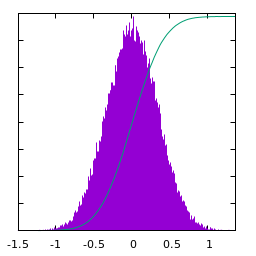
\includegraphics{l256_h.png} &
	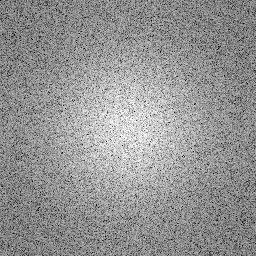
\includegraphics{l256_f.png} &
	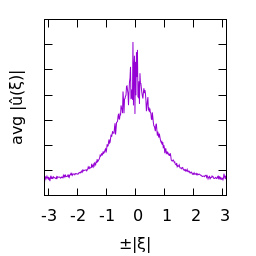
\includegraphics{l256_p.png} \\
	$u(x)$ &
	histogram of~$u$ &
	$\log|\hat u(\xi)|$ &
	average spectral profile
\end{tabular}
%SCRIPT plambda zero:256x256 randg |blur l 1 - l256.tiff
%SCRIPT qauto -p 0.1 l256.tiff l256.png &
%SCRIPT plambda l256.tiff 'x%a x%i - 300 / >1 x <1 / round <1 *' | ghisto -p | \
%SCRIPT        sed 's/cairo/cairo enhanced font "Verdana,8" size 256,256/' |\
%SCRIPT        gnuplot > l256_h.png &
%SCRIPT fft<l256.tiff|fftshift|plambda 'vnorm 1 + log'|qauto -p .1 - l256_f.png&
%SCRIPT (printf 'set term pngcairo size 256,256\nset format y ""\nset xlabel "±|ξ|"\nset ylabel "avg |û(ξ)|"\n'; fft <l256.tiff|fftshift|plambda 'vnorm'|cline nan|sed 's/data//g')|gnuplot > l256_p.png &


White gaussian noise blurred by a Disk kernel:

\begin{tabular}{cccc}
	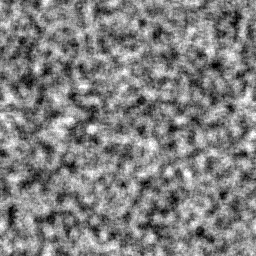
\includegraphics{d256.png} &
	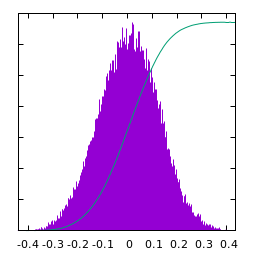
\includegraphics{d256_h.png} &
	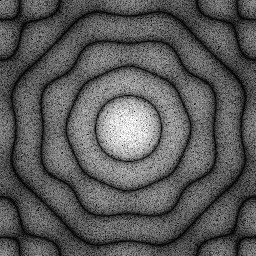
\includegraphics{d256_f.png} &
	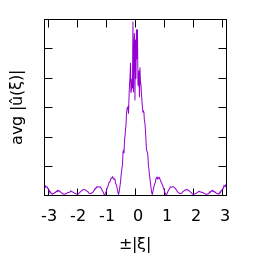
\includegraphics{d256_p.png} \\
	$u(x)$ &
	histogram of~$u$ &
	$\log|\hat u(\xi)|$ &
	average spectral profile
\end{tabular}
%SCRIPT plambda zero:256x256 randg |blur disk 4.5 - d256.tiff
%SCRIPT qauto -p 0.1 d256.tiff d256.png &
%SCRIPT plambda d256.tiff 'x%a x%i - 300 / >1 x <1 / round <1 *' | ghisto -p | \
%SCRIPT        sed 's/cairo/cairo enhanced font "Verdana,8" size 256,256/' |\
%SCRIPT        gnuplot > d256_h.png &
%SCRIPT fft<d256.tiff|fftshift|plambda 'vnorm 1 + log'|qauto -p .1 - d256_f.png&
%SCRIPT (printf 'set term pngcairo size 256,256\nset format y ""\nset xlabel "±|ξ|"\nset ylabel "avg |û(ξ)|"\n'; fft <d256.tiff|fftshift|plambda 'vnorm'|cline nan|sed 's/data//g')|gnuplot > d256_p.png &


White gaussian noise blurred by a Square kernel:

\begin{tabular}{cccc}
	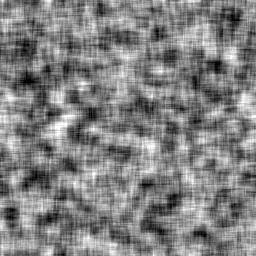
\includegraphics{s256.png} &
	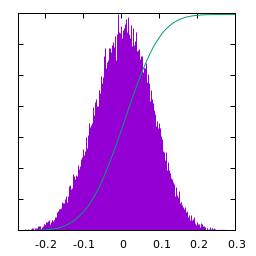
\includegraphics{s256_h.png} &
	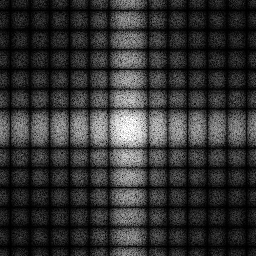
\includegraphics{s256_f.png} &
	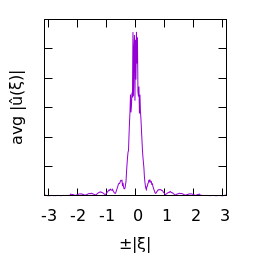
\includegraphics{s256_p.png} \\
	$u(x)$ &
	histogram of~$u$ &
	$\log|\hat u(\xi)|$ &
	average spectral profile
\end{tabular}
%SCRIPT plambda zero:256x256 randg |blur square 14 - s256.tiff
%SCRIPT qauto -p 0.1 s256.tiff s256.png
%SCRIPT plambda s256.tiff 'x%a x%i - 300 / >1 x <1 / round <1 *' | ghisto -p | \
%SCRIPT        sed 's/cairo/cairo enhanced font "Verdana,8" size 256,256/' |\
%SCRIPT        gnuplot > s256_h.png &
%SCRIPT fft<s256.tiff|fftshift|plambda 'vnorm 1 + log'|qauto -p .1 - s256_f.png&
%SCRIPT (printf 'set term pngcairo size 256,256\nset format y ""\nset xlabel "±|ξ|"\nset ylabel "avg |û(ξ)|"\n'; fft <s256.tiff|fftshift|plambda 'vnorm'|cline nan|sed 's/data//g')|gnuplot > s256_p.png &



\section{Colored gaussian noise}

When the spectrum of noise decays as a power-law, we say that it is
``colored'' noise.  The exponent~$\alpha$ of the power law determines its
color.  The particular case of~$\alpha=0$ corresponds to white noise (a flat
spectrum).


\begin{tabular}{lll}
	
\includegraphics{purple.png} &
	
\includegraphics{blue.png} &
	
\includegraphics{white2.png} \\
	$\alpha=2$ purple &
	$\alpha=1$ blue &
	$\alpha=0$ white \\
	$\phantom{a}$ &&\\
	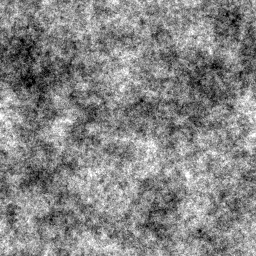
\includegraphics{pink.png} &
	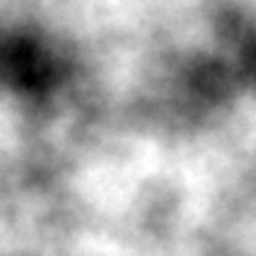
\includegraphics{brown.png} &
	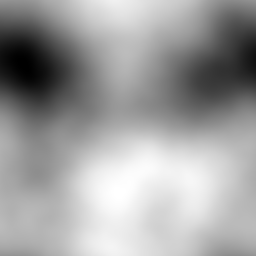
\includegraphics{smooth.png} \\
	$\alpha=-1$ pink &
	$\alpha=-2$ brown &
	$\alpha=-3$ smooth  \\
\end{tabular}
%SCRIPT plambda zero:256x256 randg -o white.tiff
%SCRIPT cat white.tiff|qauto -p 0.1 - white2.png &
%SCRIPT cat white.tiff|fft|plambda ':R 2 ^ *'|ifft|qauto -p 0.1 - purple.png &
%SCRIPT cat white.tiff|fft|plambda ':R 1 ^ *'|ifft|qauto -p 0.1 - blue.png &
%SCRIPT cat white.tiff|fft|plambda ':R -1 ^ *'|ifft|qauto -p 0.1 - pink.png &
%SCRIPT cat white.tiff|fft|plambda ':R -2 ^ *'|ifft|qauto -p 0.1 - brown.png &
%SCRIPT cat white.tiff|fft|plambda ':R -3 ^ *'|ifft|qauto -p 0.1 - smooth.png &


Statistics of Pink noise ($\alpha=-1$):

\begin{tabular}{cccc}
	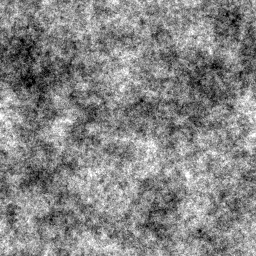
\includegraphics{KK-1.png} &
	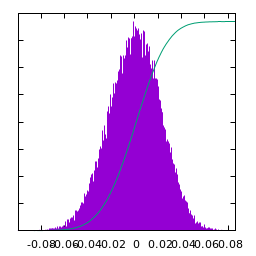
\includegraphics{KK-1_h.png} &
	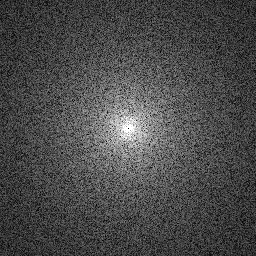
\includegraphics{KK-1_f.png} &
	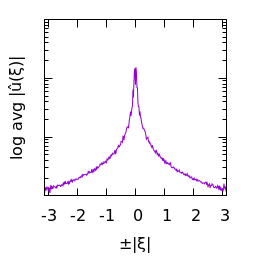
\includegraphics{KK-1_p.png} \\
	$u(x)$ &
	histogram of~$u$ &
	$\log|\hat u(\xi)|$ &
	average spectral profile
\end{tabular}
%SCRIPT plambda zero:256x256 randg|fft|plambda ':R -1 ^ *'|ifft >KK-1.tiff
%SCRIPT qauto -p 0.1 KK-1.tiff KK-1.png &
%SCRIPT plambda KK-1.tiff 'x%a x%i - 300 / >1 x <1 / round <1 *' | ghisto -p | \
%SCRIPT        sed 's/cairo/cairo enhanced font "Verdana,8" size 256,256/' |\
%SCRIPT        gnuplot > KK-1_h.png &
%SCRIPT fft<KK-1.tiff|fftshift|plambda 'vnorm 1 + log'|qauto -p .1 - KK-1_f.png&
%SCRIPT (printf 'set term pngcairo size 256,256\nset format y ""\nset xlabel "±|ξ|"\nset ylabel "log avg |û(ξ)|"\nset logscale y\n'; fft <KK-1.tiff|fftshift|plambda 'vnorm'|cline nan|sed 's/data//g')|gnuplot > KK-1_p.png &



Statistics of Brown noise ($\alpha=-2$):

\begin{tabular}{cccc}
	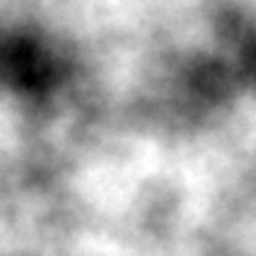
\includegraphics{KK-2.png} &
	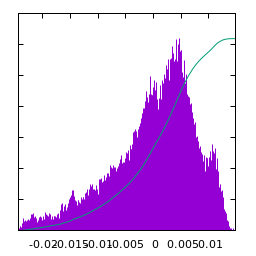
\includegraphics{KK-2_h.png} &
	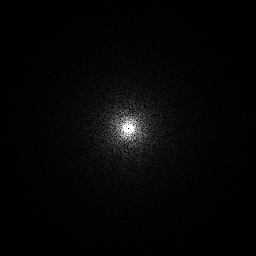
\includegraphics{KK-2_f.png} &
	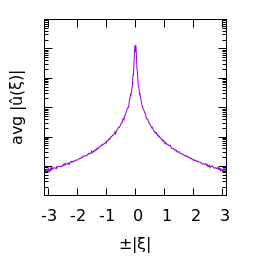
\includegraphics{KK-2_p.png} \\
	$u(x)$ &
	histogram of~$u$ &
	$\log|\hat u(\xi)|$ &
	average spectral profile
\end{tabular}
%SCRIPT plambda zero:256x256 randg|fft|plambda ':R -2 ^ *'|ifft >KK-2.tiff
%SCRIPT qauto -p 0.1 KK-2.tiff KK-2.png &
%SCRIPT plambda KK-2.tiff 'x%a x%i - 300 / >1 x <1 / round <1 *' | ghisto -p | \
%SCRIPT        sed 's/cairo/cairo enhanced font "Verdana,8" size 256,256/' | \
%SCRIPT        gnuplot > KK-2_h.png &
%SCRIPT fft<KK-2.tiff|fftshift|plambda 'vnorm 1 + log'|qauto -p .1 - KK-2_f.png&
%SCRIPT (printf 'set term pngcairo size 256,256\nset format y ""\nset xlabel "±|ξ|"\nset ylabel "avg |û(ξ)|"\nset logscale y\n'; fft <KK-2.tiff|fftshift|plambda 'vnorm'|cline nan|sed 's/data//g')|gnuplot > KK-2_p.png &

Statistics of Smooth noise ($\alpha=-3$):

\begin{tabular}{cccc}
	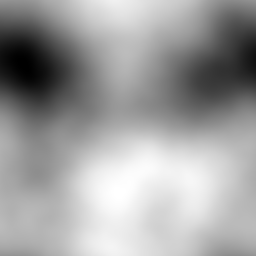
\includegraphics{KK-3.png} &
	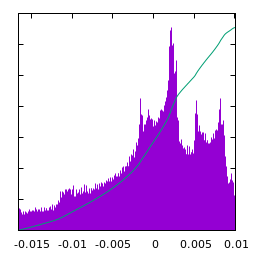
\includegraphics{KK-3_h.png} &
	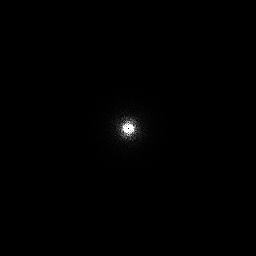
\includegraphics{KK-3_f.png} &
	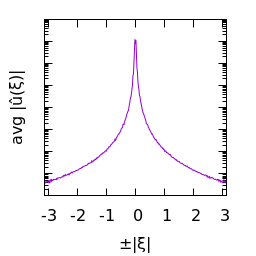
\includegraphics{KK-3_p.png} \\
	$u(x)$ &
	histogram of~$u$ &
	$\log|\hat u(\xi)|$ &
	average spectral profile
\end{tabular}
%SCRIPT plambda zero:256x256 randg|fft|plambda ':R -3 ^ *'|ifft >KK-3.tiff
%SCRIPT qauto -p 0.1 KK-3.tiff KK-3.png &
%SCRIPT plambda KK-3.tiff 'x%a x%i - 300 / >1 x <1 / round <1 *' | ghisto -p | \
%SCRIPT        sed 's/cairo/cairo enhanced font "Verdana,8" size 256,256/' | \
%SCRIPT        gnuplot > KK-3_h.png &
%SCRIPT fft<KK-3.tiff|fftshift|plambda 'vnorm 1 + log'|qauto -p .1 - KK-3_f.png&
%SCRIPT (printf 'set term pngcairo size 256,256\nset format y ""\nset xlabel "±|ξ|"\nset ylabel "avg |û(ξ)|"\nset logscale y\n'; fft <KK-3.tiff|fftshift|plambda 'vnorm'|cline nan|sed 's/data//g')|gnuplot > KK-3_p.png &


Statistics of Blue noise ($\alpha=1$):

\begin{tabular}{cccc}
	
\includegraphics{KK+1.png} &
	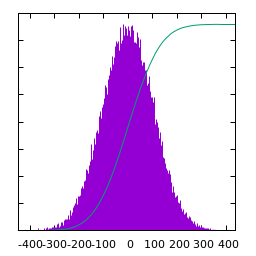
\includegraphics{KK+1_h.png} &
	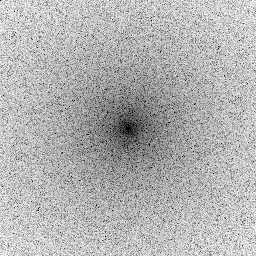
\includegraphics{KK+1_f.png} &
	\includegraphics{KK+1_p.png} \\
	$u(x)$ &
	histogram of~$u$ &
	$\log|\hat u(\xi)|$ &
	average spectral profile
\end{tabular}
%SCRIPT plambda zero:256x256 randg|fft|plambda ':R 1 ^ *'|ifft >KK+1.tiff
%SCRIPT qauto -p 0.1 KK+1.tiff KK+1.png &
%SCRIPT plambda KK+1.tiff 'x%a x%i - 300 / >1 x <1 / round <1 *' | ghisto -p | \
%SCRIPT        sed 's/cairo/cairo enhanced font "Verdana,8" size 256,256/' | \
%SCRIPT        gnuplot > KK+1_h.png &
%SCRIPT fft<KK+1.tiff|fftshift|plambda 'vnorm 1 + log'|qauto -p .1 - KK+1_f.png&
%SCRIPT (printf 'set term pngcairo size 256,256\nset format y ""\nset xlabel "±|ξ|"\nset ylabel "avg |û(ξ)|"\nset logscale y\n'; fft <KK+1.tiff|fftshift|plambda 'vnorm'|cline nan|sed 's/data//g')|gnuplot > KK+1_p.png &


Statistics of Purple noise ($\alpha=2$):

\begin{tabular}{cccc}
	\includegraphics{KK+2.png} &
	\includegraphics{KK+2_h.png} &
	\includegraphics{KK+2_f.png} &
	\includegraphics{KK+2_p.png} \\
	$u(x)$ &
	histogram of~$u$ &
	$\log|\hat u(\xi)|$ &
	average spectral profile
\end{tabular}
%SCRIPT plambda zero:256x256 randg|fft|plambda ':R 2 ^ *'|ifft >KK+2.tiff
%SCRIPT qauto -p 0.1 KK+2.tiff KK+2.png &
%SCRIPT plambda KK+2.tiff 'x%a x%i - 300 / >1 x <1 / round <1 *' | ghisto -p | \
%SCRIPT        sed 's/cairo/cairo enhanced font "Verdana,8" size 256,256/' | \
%SCRIPT        gnuplot > KK+2_h.png &
%SCRIPT fft<KK+2.tiff|fftshift|plambda 'vnorm 1 + log'|qauto -p .1 - KK+2_f.png&
%SCRIPT (printf 'set term pngcairo size 256,256\nset format y ""\nset xlabel "±|ξ|"\nset ylabel "avg |û(ξ)|"\nset logscale y\n'; fft <KK+2.tiff|fftshift|plambda 'vnorm'|cline nan|sed 's/data//g')|gnuplot > KK+2_p.png &


%SCRIPT wait

% vim:set tw=77 filetype=tex spell spelllang=en:
